\documentclass[crop=false]{standalone}
%\documentclass{standalone}
\usepackage{tikz} % To generate the plot from csv
\usepackage{pgfplots}
\usepackage{graphicx}
\usepackage{booktabs}
\usepackage{subfig}
\usepackage{float}
\usepackage[section]{placeins} % getting figures below sections
\usepackage{blindtext}
\usepackage{siunitx}
\usepgfplotslibrary{units} % Allows to enter the units nicely
\usetikzlibrary{external} %https://tex.stackexchange.com/questions/1460/script-to-automate-externalizing-tikz-graphics
\tikzexternalize[prefix=savedfigures/]

\pgfplotsset{compat=newest} % Allows to place the legend below plot
\usepackage{pgfplotstable}
\usepgfplotslibrary{statistics}

% #################### Function definition for box plots read table ##################\
\makeatletter
\pgfplotsset{
	boxplot prepared from table/.code={
		\def\tikz@plot@handler{\pgfplotsplothandlerboxplotprepared}%
		\pgfplotsset{
			/pgfplots/boxplot prepared from table/.cd,
			#1,
		}
	},
	/pgfplots/boxplot prepared from table/.cd,
	table/.code={\pgfplotstablecopy{#1}\to\boxplot@datatable},
	row/.initial=0,
	make style readable from table/.style={
		#1/.code={
			\pgfplotstablegetelem{\pgfkeysvalueof{/pgfplots/boxplot prepared from table/row}}{##1}\of\boxplot@datatable
			\pgfplotsset{boxplot/#1/.expand once={\pgfplotsretval}}
		}
	},
	make style readable from table=lower whisker,
	make style readable from table=upper whisker,
	make style readable from table=lower quartile,
	make style readable from table=upper quartile,
	make style readable from table=median,
	make style readable from table=average,
	make style readable from table=lower notch,
	make style readable from table=upper notch
}
\makeatother
\begin{document}

\section{2 1 Mandl6 GA Crossover 20210716 115805}

% ######################## UTRP GA Crossover operators applied ######################## 
\begin{figure} 
\centering 
\tikzsetnextfilename{UTRP_NSGAII_BP_crossover_funcs_phd} 
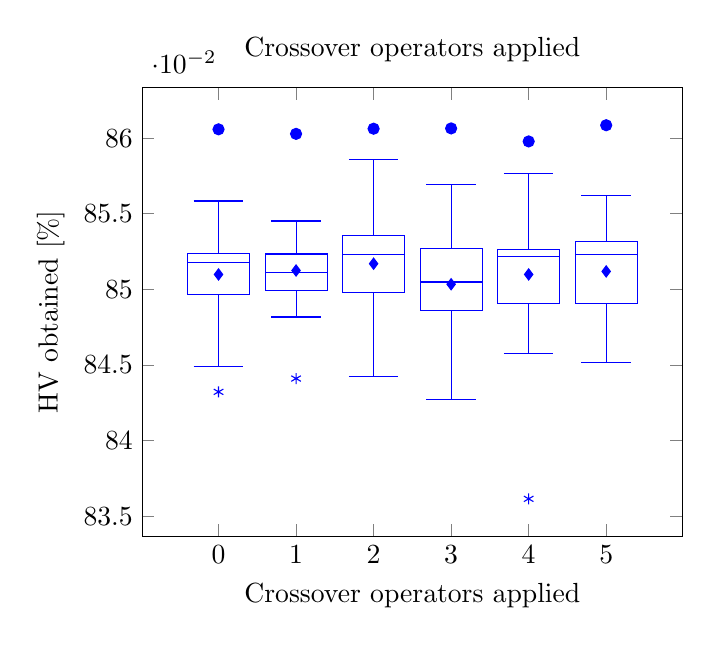
\begin{tikzpicture} 
\begin{axis}[ 
title={Crossover operators applied}, 
boxplot/draw direction=y, 
xtick={1,2,3,4,5,6}, 
xticklabels={0,1,2,3,4,5}, 
x tick label style={rotate=0, align=center}, 
xlabel={Crossover operators applied}, 
scaled y ticks={base 10:2}, %y tick label style={/pgf/number format/.cd,fixed,precision=3, zerofill}, 
ylabel={HV obtained [\%]}, 
] 

% ############## Crossover=0 ################## 
\addplot[boxplot, mark=asterisk, 
boxplot prepared={ 
lower whisker=0.84489, 
upper whisker=0.85584, 
lower quartile=0.84966, 
upper quartile=0.85235, 
median=0.85177, 
average=0.85099}, 
color = blue, solid, area legend] 
coordinates {
(1,0.84323)}; 
\addplot[only marks,mark=*,color = blue]coordinates{(1,0.86058)}; 

% ############## Crossover=1 ################## 
\addplot[boxplot, mark=asterisk, 
boxplot prepared={ 
lower whisker=0.84818, 
upper whisker=0.85452, 
lower quartile=0.84994, 
upper quartile=0.85234, 
median=0.85114, 
average=0.85125}, 
color = blue, solid, area legend] 
coordinates {
(2,0.84411)}; 
\addplot[only marks,mark=*,color = blue]coordinates{(2,0.86028)}; 

% ############## Crossover=2 ################## 
\addplot[boxplot, mark=asterisk, 
boxplot prepared={ 
lower whisker=0.84427, 
upper whisker=0.85859, 
lower quartile=0.84981, 
upper quartile=0.85355, 
median=0.85233, 
average=0.8517}, 
color = blue, solid, area legend] 
coordinates {}; 
\addplot[only marks,mark=*,color = blue]coordinates{(3,0.86062)}; 

% ############## Crossover=3 ################## 
\addplot[boxplot, mark=asterisk, 
boxplot prepared={ 
lower whisker=0.84273, 
upper whisker=0.85693, 
lower quartile=0.84862, 
upper quartile=0.85269, 
median=0.85049, 
average=0.85034}, 
color = blue, solid, area legend] 
coordinates {}; 
\addplot[only marks,mark=*,color = blue]coordinates{(4,0.86064)}; 

% ############## Crossover=4 ################## 
\addplot[boxplot, mark=asterisk, 
boxplot prepared={ 
lower whisker=0.84577, 
upper whisker=0.85767, 
lower quartile=0.84904, 
upper quartile=0.85266, 
median=0.85215, 
average=0.85099}, 
color = blue, solid, area legend] 
coordinates {
(5,0.83616)}; 
\addplot[only marks,mark=*,color = blue]coordinates{(5,0.85978)}; 

% ############## Crossover=5 ################## 
\addplot[boxplot, mark=asterisk, 
boxplot prepared={ 
lower whisker=0.84519, 
upper whisker=0.85618, 
lower quartile=0.84907, 
upper quartile=0.85319, 
median=0.85228, 
average=0.85119}, 
color = blue, solid, area legend] 
coordinates {}; 
\addplot[only marks,mark=*,color = blue]coordinates{(6,0.86085)}; 

\end{axis}
\end{tikzpicture}
\end{figure} 
\begin{table}
\centering
\caption{Legend for the boxplot.}
\begin{tabular}{ll}
\toprule
 Index &                                     Name \\
\midrule
     0 &                                  Mumford \\
     1 &                     Unseen\_probabilistic \\
     2 &              Mumford\_replace\_subsets\_ksp \\
     3 & Unseen\_probabilistic\_replace\_subsets\_ksp \\
     4 &                  Mumford\_replace\_subsets \\
     5 &     Unseen\_probabilistic\_replace\_subsets \\
\bottomrule
\end{tabular}
\end{table}

\end{document}
